% Created 2024-05-15 Wed 03:05
% Intended LaTeX compiler: pdflatex
\documentclass[a4paper]{article}
\usepackage[utf8]{inputenc}
\usepackage[T1]{fontenc}
\usepackage{graphicx}
\usepackage{longtable}
\usepackage{wrapfig}
\usepackage{rotating}
\usepackage[normalem]{ulem}
\usepackage{amsmath}
\usepackage{amssymb}
\usepackage{capt-of}
\usepackage{hyperref}
\usepackage{breakcites}
\usepackage{paralist}
\usepackage{amsmath}
\usepackage{biblatex}
\usepackage{hyperref}
\usepackage{graphicx}
\usepackage{caption}
\usepackage{booktabs}
\usepackage[T1]{fontenc}
\usepackage{tgbonum}
\let\itemize\compactitem
\let\description\compactdesc
\let\enumerate\compactenum
\author{Dimitrios Papachistopoulos}
\date{\today}
\title{Investigations of the galaxies of the LCV\\\medskip
\large Finding the normalization constant of SFR_{del} and the relations between the various masses of the Galaxies}
\hypersetup{
 pdfauthor={Dimitrios Papachistopoulos},
 pdftitle={Investigations of the galaxies of the LCV},
 pdfkeywords={},
 pdfsubject={},
 pdfcreator={Emacs 29.3 (Org mode 9.6.24)}, 
 pdflang={English}}
\begin{document}

\maketitle

\begin{abstract}
The paper investigates the properties of galaxies in the Local Cosmological Volume (LCV), using the Catalogue of Neighboring Galaxies(Karachentsev, Igor D. and Makarov, Dmitry I. and Kaisina, Elena I., 2013) and its updated version from the ``Catalog \& Atlas of the LV galaxies'' database(, ). The properties studied include the galaxy types, their various masses, the star formation rates (SFRs) and the star formation timescale \(\tau\), gas depletion timescale \(\tau_g\) and the star formation time \(t_{sf}\). The paper aims to understand the distribution and correlation of these properties in the sample of galaxies in the LCV, and how they relate to current astrophysical theories.
\end{abstract}

\section{The Galaxies in the Local Cosmological Volume (LCV)}
\label{sec:orga2f0b32}

The Catalogue of Neigbouring Galaxies (Karachentsev, Igor D. and Makarov  et al. 2013(Karachentsev, Igor D. and Makarov, Dmitry I. and Kaisina, Elena I., 2013)) and its updated version from the ``Catalog \& Atlas of the LV galaxies'' databas(, )  are used to extract the K-band luminosities, the types of the galaxies, the mass within the Holmberg radius (M26), the Hydrogen masses of the galaxies (\(M_{HI}\)) and the SFRs based on integrated  H and far-ultraviolet (FUV) measurments for galaxies within a distance of \(\approx 11\) Mpc.

\subsection{How are the galaxies chosen}
\label{sec:orgde10150}

According to (Kraan-Korteweg, R. C. and Tammann, G. A., 1979) the Local Cosmological Volume is defined as the galaxies inside the radius of 10 Mpc and having radial velocities with respect to centroid of the Local Group \(V_{lg} \le 500 \, km \cdot s^{-1}\). However, this assumed a Hubble constant of \(H_0 = 50\, km \cdot s^{-1}\).

\begin{enumerate}
\item \textbf{Initial Selection Criteria}: Galaxies within a 10 Mpc radius were initially selected based on a radial velocity limit (VLG) of 500 km/s, considering a Hubble parameter (H0) of 50 km/s/Mpc.

\item \textbf{Updated Criteria}: To accommodate the revised H0 value of 73 km/s/Mpc, the VLG limit needs to be raised to 730 km/s.

\item \textbf{Local Velocity Field}: The presence of the Virgo cluster and the Local Void introduces additional velocity components, complicating distance estimation based solely on radial velocities.

\item \textbf{Peculiar Motions}: Collective motions within large-scale structures can introduce peculiar velocities, complicating distance estimation.

\item \textbf{Distance Measurement Methods}: Direct distance measurements using methods like the tip of the red giant branch (TRGB) provide accurate distances but are resource-intensive, requiring extensive observation time with instruments like the Hubble Space Telescope (HST).

\item \textbf{Inclusion Criteria}: Galaxies are included based on either radial velocities or distance estimates, considering the limitations and uncertainties in both methods.

\item \textbf{Extension to 11 Mpc}: Galaxies with distance estimates beyond 10 Mpc may still be included due to uncertainties in distance measurements and the potential influence of coherent motions and large-scale structures.

\item \textbf{Sample Composition}: The LV sample comprises \texttt{1448} galaxies, with considerations for galaxies near the boundaries of the selection criteria and the potential influence of measurement errors.

\begin{center}
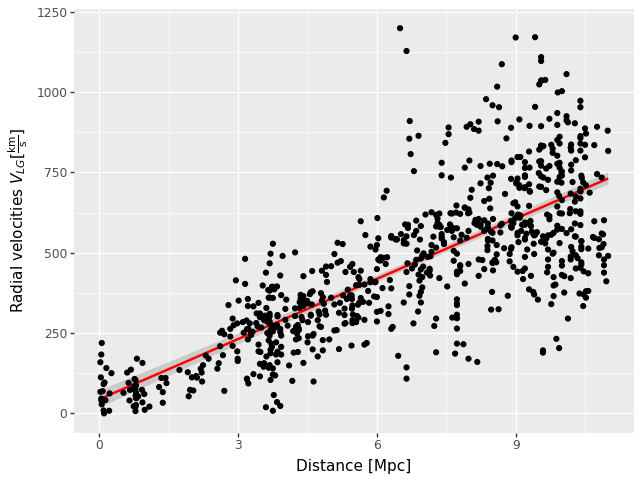
\includegraphics[width=.9\linewidth]{figure/hubble.png}
\end{center}
\end{enumerate}


\subsection{Mapping the galaxies}
\label{sec:orgedc2b80}

Because matplotlib needs the coordinates in radians and between \(-\pi\) and \(\pi\)
and, not 0 and \(2\pi\), we have to convert coordinates.

\begin{center}
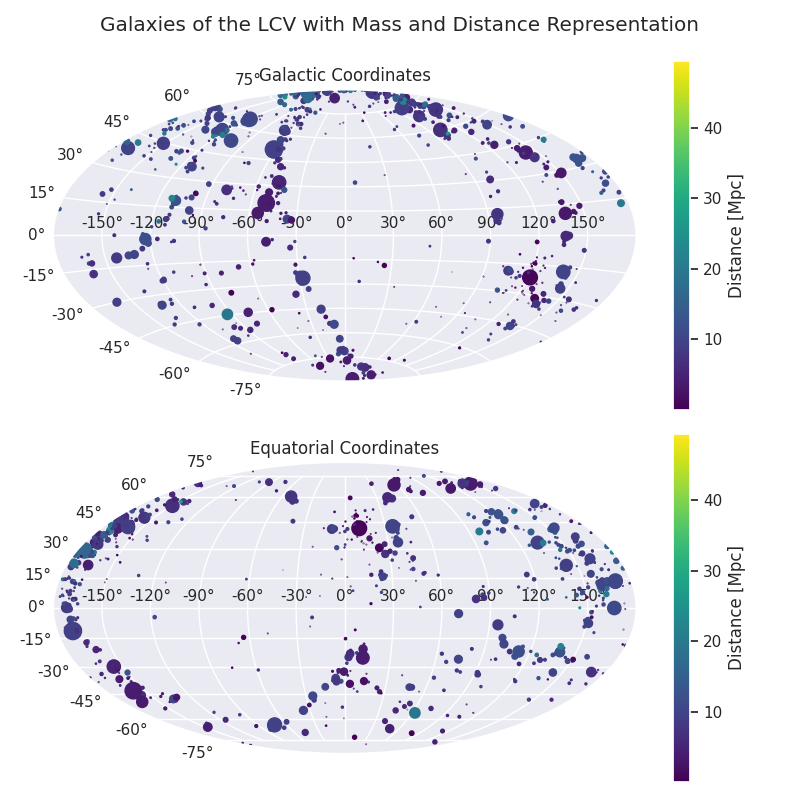
\includegraphics[width=.9\linewidth]{figure/mapping.png}
\end{center}


\subsection{Types of galaxies}
\label{sec:org026d262}

Using the dataset of \texttt{1448}
galaxies, we can study the morphology of the galaxies in the LCV

\subsubsection{Morphology}
\label{sec:org66e126b}
\begin{center}
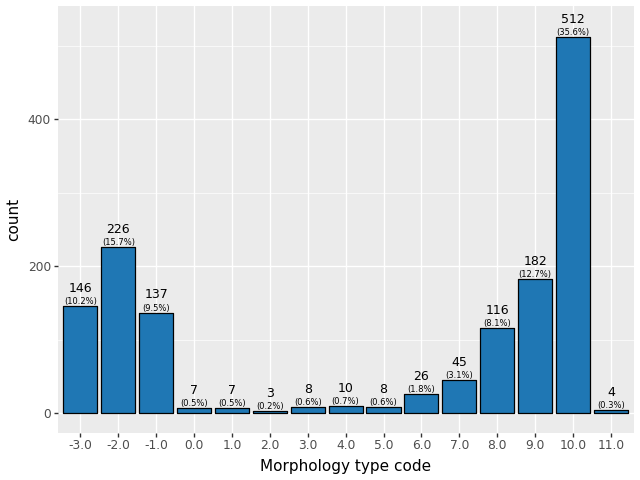
\includegraphics[width=.9\linewidth]{./figure/Types.png}
\end{center}






\begin{enumerate}
\item Morphology of dwarf galaxies
\label{sec:org9759d71}


\begin{center}
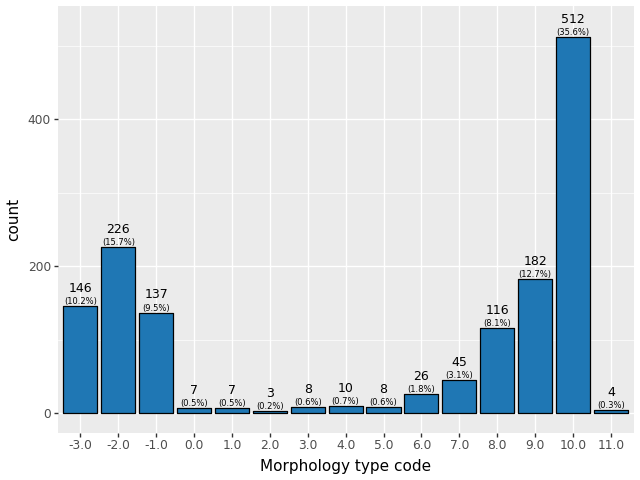
\includegraphics[width=.9\linewidth]{./figure/Types.png}
\end{center}



\item Dwarf galaxy surface brightness morphology
\label{sec:org80a0b66}

\begin{center}
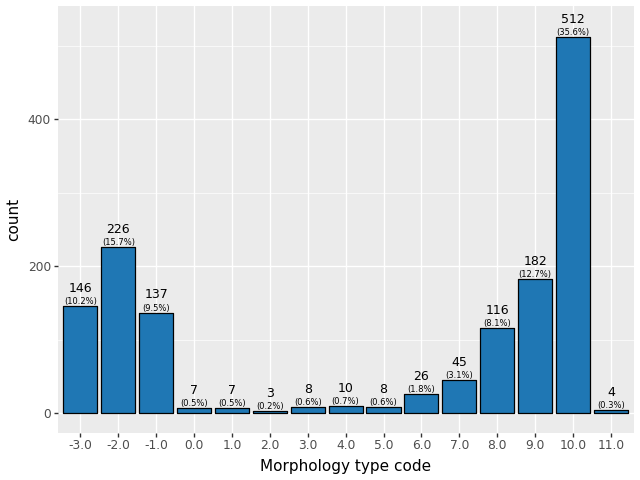
\includegraphics[width=.9\linewidth]{./figure/Types.png}
\end{center}
\end{enumerate}


\section{Understanding the Data}
\label{sec:org7cd3cde}

The catalog consists of 8 tables

\begin{enumerate}
\item Catalog of Nearby Galaxies
\item Global Parameters of the Nearby Galaxies
\item List of Apparent Magnitudes
\item List of Heliocentric Velocities
\item List of Inner Kinematics
\item List of Distances
\item List of the nearby galaxies with measured SFR
\item List of Bibliographic References
\end{enumerate}

We want several measurments from those lists so we will join them according to the name of the galaxy.

This catalog consists of \texttt{1449} galaxies

\subsection{Understanding the limit flags}
\label{sec:org3ad49c4}

Some of those values contain limit flags, which we will mask for our present analysis. However, those values will be shown in the plots, and afterwards will be compared with the theoretical values.

\begin{verbatim}
All masks in l_FUVmag are also masks in FUVmag
All masks in l_Hamag are also masks in Hamag
All masks in f_Kmag are also masks in Kmag
All masks in l_21mag are also masks in 21mag
We have no mask for f_Dis
All masks in l_logMHI are also masks in logMHI
All masks in l_mag_B are also masks in mag_B
All masks in l_mag_FUV are also masks in mag_FUV
All masks in l_mag_HI are also masks in mag_HI
All masks in l_mag_Ha are also masks in mag_Ha
All masks in l_mag_Ks are also masks in mag_Ks
All masks in l_SFRHa are also masks in SFRHa
All masks in l_PHa are also masks in PHa
All masks in l_FHa are also masks in FHa
All masks in l_SFRFUV are also masks in SFRFUV
All masks in l_PFUV are also masks in PFUV
All masks in l_FFUV are also masks in FFUV
\end{verbatim}




\section{Standarized constants}
\label{sec:org7f042ce}

We should use some standart consistent values for our analysis.

\begin{enumerate}
\item According to (Speagle, Joshua S. and Steinhardt, Charles L. and Capak, Peter L. and Silverman, John D., 2014) and(Kroupa, P and Haslbauer, M and Banik, I and Nagesh, S T and Pflamm-Altenburg, J, 2020) the \(t_{sf} = 12\, Gyr\) represents a strong and consistent constraint of galaxy evolution, across many studies. While other researchers adopt a t\textsubscript{sf}= 13.6 Gyr(Haslbauer, Moritz and Kroupa, Pavel and Jerabkova, Tereza, 2023), we use the 12 Gyr assumption following the framework of SP14
\item \(\zeta =\) accommodates mass-loss through stellar evolution. According to the IGIMF theory the galaxies of the the LCV are expected to have 1< \(\zeta\) <1.3, so by adopting \(\zeta =1.3\) we are working conservatively
\item Main Sequence z = 5
\end{enumerate}

\section{Calculations for values that we need}
\label{sec:orgea354e0}


\subsection{Total stellar masses, the total gas mass and total barionic of the galaxies}
\label{sec:orgf921de0}

The \(MHI\) can be converted to the total mass of the gas of the galaxy using the equation \(M_g=1.33\, MHI\)


The K-band values are converted to the total Stellar Masses of each galaxy according to the mass-to-light ratio of 0.6 (\(M_\odot/Lum\))(Lelli, Federico and McGaugh, Stacy S. and Schombert, James M., 2016)

\begin{verbatim}
name = StellarMass
dtype = float64
unit = solMass
description = Linear K_S_ band luminosity
class = MaskedQuantity
n_bad = 12
length = 1448
\end{verbatim}


The total barionic mass can be calcuated as the sum of the total gas mass of the galaxy with the Stellar mass

\begin{verbatim}
name = BarMass
dtype = float64
unit = solMass
description = Linear hydrogen mass
class = MaskedQuantity
n_bad = 513
length = 1448
\end{verbatim}

\subsubsection{Ratio of M\textsubscript{g} and StellarMass}
\label{sec:org6ebf887}

\begin{verbatim}
/home/dp/.local/lib/python3.10/site-packages/astropy/utils/masked/core.py:879: RuntimeWarning: divide by zero encountered in divide
name = mass_ratio
dtype = float64
description = Linear hydrogen mass
class = MaskedQuantity
mean = 2.13272
std = 3.81136
min = 7.51105e-05
max = 58.3043
n_bad = 513
length = 1448
\end{verbatim}

Histogram of dt[``mass\textsubscript{ratio}'']

\subsection{Color index}
\label{sec:orgdc5850f}

Here we calculate the color indexes <FUV-B>

The lower the value, the bluer the stars, thus the younger the star populations

\begin{center}
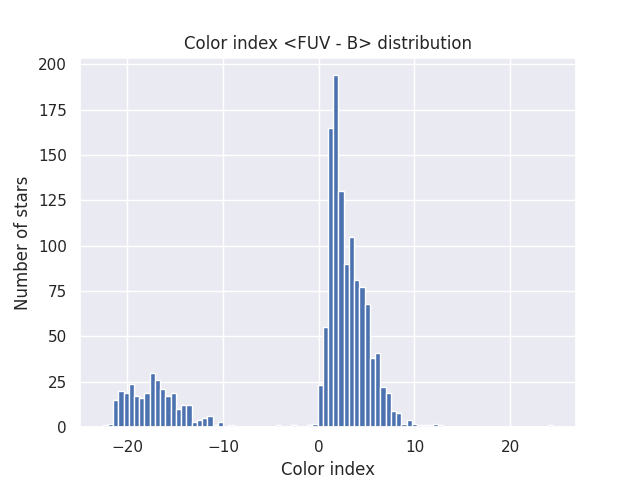
\includegraphics[width=.9\linewidth]{./figure/color_index.png}
\end{center}

\subsection{Fixing the SFRs}
\label{sec:orgbc555ea}


\subsubsection{SFR units}
\label{sec:orgbb95c1a}

\begin{verbatim}
None
\end{verbatim}
\subsubsection{log to linear}
\label{sec:org61b8988}

they are the power in logarithmic scale. SO lets fix them


\begin{verbatim}
name = SFRFUV
dtype = float64
unit = solMass / yr
class = Quantity
n_bad = 321
length = 1448
\end{verbatim}


\begin{verbatim}
<QTable length=1448>
 name          mean                 std                    min                  max      
------ -------------------- -------------------- ------------------------ ---------------
SFRFUV 2.27435 solMass / yr 4.13466 solMass / yr 2.13796e-10 solMass / yr 10 solMass / yr
 SFRHa 4.97642 solMass / yr 4.94957 solMass / yr 1.38038e-10 solMass / yr 10 solMass / yr
\end{verbatim}


\subsection{SFR\textsubscript{0}}
\label{sec:org10b773e}


Now we have to calculate the total SFR from the equation:

$$
    SFR_o=\frac{SFR_{FUV}+SFR_{Ha}}{2}
$$

if we have both the SFR. If we only have one of them then:

$$
    SFR_{0}=SFR_{i},\ \text{if } SFR_{j}=0,\ i\neq j,\ i,j=SFR_{FUV},\, SFR_{Ha}
$$


create the average SFR\textsubscript{0} from SFRHa SFRFUV with np.ma.average

\begin{verbatim}
/home/dp/.local/lib/python3.10/site-packages/numpy/core/fromnumeric.py:3504: RuntimeWarning: Mean of empty slice.
/home/dp/.local/lib/python3.10/site-packages/numpy/core/_methods.py:121: RuntimeWarning: invalid value encountered in divide
<QTable length=1448>
 name           mean                   std                    min                    max          n_bad
------ ---------------------- --------------------- ------------------------ -------------------- -----
 SFR_0 0.0722542 solMass / yr 0.316258 solMass / yr 1.75917e-10 solMass / yr 4.38718 solMass / yr   190
SFRFUV   2.27435 solMass / yr  4.13466 solMass / yr 2.13796e-10 solMass / yr      10 solMass / yr     0
 SFRHa   4.97642 solMass / yr  4.94957 solMass / yr 1.38038e-10 solMass / yr      10 solMass / yr     0
\end{verbatim}



\begin{verbatim}
name = SFRHa
mean = 4.97642 solMass / yr
std = 4.94957 solMass / yr
min = 1.38038e-10 solMass / yr
max = 10 solMass / yr
n_bad = 712
length = 1448
None
\end{verbatim}

\subsection{Applying the cut SFR\textsubscript{0} >= 1e-3 solMass/yr}
\label{sec:org8549e88}

keep only the SFR\textsubscript{0} data were >1e-3

\begin{verbatim}
WARNING: column logKLum has a unit but is kept as a MaskedColumn as an attempt to convert it to Quantity failed with:
UnitTypeError("MaskedQuantity instances require normal units, not <class 'astropy.units.function.logarithmic.DexUnit'> instances.") [astropy.table.table]
WARNING: column logM26 has a unit but is kept as a MaskedColumn as an attempt to convert it to Quantity failed with:
UnitTypeError("MaskedQuantity instances require normal units, not <class 'astropy.units.function.logarithmic.DexUnit'> instances.") [astropy.table.table]
WARNING: column logMHI has a unit but is kept as a MaskedColumn as an attempt to convert it to Quantity failed with:
UnitTypeError("MaskedQuantity instances require normal units, not <class 'astropy.units.function.logarithmic.DexUnit'> instances.") [astropy.table.table]
name = SFR_0
dtype = float64
unit = solMass / yr
class = Quantity
n_bad = 0
length = 607
None
\end{verbatim}

\begin{verbatim}
<QTable length=607>
 name           mean                  std                    min                    max         
------ --------------------- --------------------- ------------------------ --------------------
 SFR_0 0.149597 solMass / yr 0.442412 solMass / yr  0.00102329 solMass / yr 4.38718 solMass / yr
SFRFUV  1.66911 solMass / yr   3.5739 solMass / yr 6.60693e-05 solMass / yr      10 solMass / yr
 SFRHa  1.95358 solMass / yr  3.81106 solMass / yr 2.04174e-05 solMass / yr      10 solMass / yr
\end{verbatim}


Histogram of SFR\textsubscript{0}

\subsection{Theoretical Average SFR}
\label{sec:org283c16a}

To calculate the average Star Formation Rate \(\overline{SFR}\) we can use the equation

$$
    \overline{SFR}=\frac{\zeta M_*}{t_{sf}}
$$

where ζ is the mass-loss through stellar evolution and we assume that \(\zeta\approx 1.3\) (see explanation in the paper`), M* is the stellar mass of each galaxy and we assume that is   \(t_{sf}=12.5\ Gyr\)

\begin{verbatim}
name = av_SFR_theor
dtype = float64
unit = solMass / yr
description = Linear K_S_ band luminosity
class = MaskedQuantity
n_bad = 1
length = 607
\end{verbatim}


\subsection{Ratio av\textsubscript{SFR}/SFR\textsubscript{0}}
\label{sec:org01c7dc6}


Now we have to calculate the ratio \(\frac{\overline{SFR}}{SFR_0}\)

\begin{verbatim}
/home/dp/.local/lib/python3.10/site-packages/astropy/utils/masked/core.py:879: RuntimeWarning: divide by zero encountered in log10
<QTable length=607>
    name      dtype          description             class         mean     std       min      max   n_bad
------------ ------- --------------------------- -------------- --------- -------- --------- ------- -----
   SFR_ratio float64 Linear K_S_ band luminosity MaskedQuantity   5.77922  45.5965 0.0325391 1054.18     1
logSFR_ratio float64 Linear K_S_ band luminosity MaskedQuantity 0.0646566 0.515905  -1.48759 3.02291     1
\end{verbatim}


log10 of ratio

Scatter color and ratio

\begin{center}
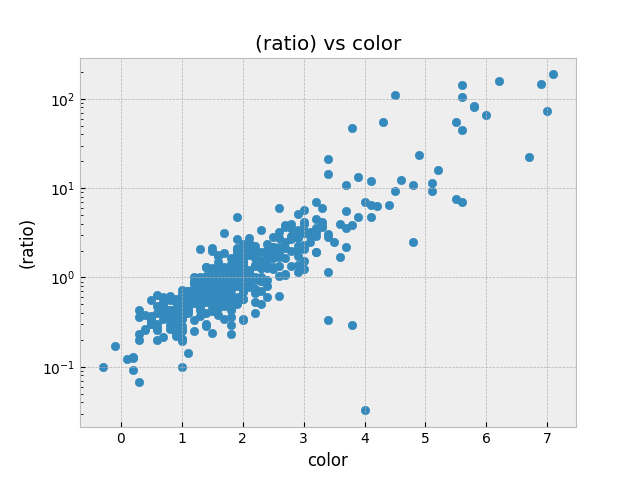
\includegraphics[width=.9\linewidth]{figure/ratio_vs_color.png}
\end{center}


\section{The Delayed-\(\tau\) model}
\label{sec:org0d51031}

``The delayed-τ model describes the SFH of a galaxy assuming that the SFRs typically rise in the early phase of galaxy evolution and gradually decline to the present time (e.g. Reddy et al. 2012; Carnall et al. 2019). In fact, Speagle et al. (2014) showed in their figures 9 and 10 that the SFH of galaxies following the main sequence of star-forming galaxies can be accurately parametrized by the delayed-τ model of the form'' (Haslbauer, Moritz and Kroupa, Pavel and Jerabkova, Tereza, 2023)


\begin{equation}
        \label{eq:SFR} SFR_{0,del}=\frac{A_{del}xe^{-x}}{\tau},\text{ where } x=\frac{tsf}{\tau}
\end{equation}

\noindent where

is the star formation time-scale, \(tsf\) is the real time of star formation in a given galaxy and \(Adel\) a normalization constant.

The average SFR is

\begin{equation}
        \label{eq:av_SFR-x} \overline{SFRdel}=\frac{Adel}{tsf}[1-(1+x)e^{-x}]
\end{equation}
and can also be defined by the present day stellar mass

\begin{equation}\label{eq:av_SFR M*}
        \overline{SFR}=\frac{\zeta M_*}{tsf}
\end{equation}

where
accommodates for mass-loss through stella evolution and This is a system of 2 equations and 3 variables

\subsection{Calculating A\textsubscript{del}}
\label{sec:orgb51a76e}

\subsubsection{Constant t\textsubscript{sf}}
\label{sec:org1f90dc5}
The observed ages of galactic discs are \(tsf≈ 12\) Gyr(Knox, R. A. and Hawkins, M. R. S. and Hambly, N. C., 1999), so assuming an approximation of \(tsf=12\) Gyr, the \(\overline{SFR_{del}}\) can be calcuated, from the equation (\ref{eq:av_SFR M*}).


After that the equation of ratio

\begin{equation} \label{eq:ratio}                                        \frac{\overline{SFRdel}}{SFR0,del}=\frac{e^x-x-1}{x^2}
\end{equation}

can be solved numerically for x and using the equations (\Ref{eq:SFR}) and (\Ref{eq:av_SFR-x}) the \(Adel\) and of each galaxy are found.

\begin{verbatim}
<QTable length=607>
    name     dtype      unit             description             class      n_bad
----------- ------- ------------ --------------------------- -------------- -----
      SFR_0 float64 solMass / yr                                   Quantity     0
  SFR_ratio float64              Linear K_S_ band luminosity MaskedQuantity     1
StellarMass float64      solMass Linear K_S_ band luminosity MaskedQuantity     1
\end{verbatim}

\subsubsection{Newton}
\label{sec:org30977fb}

\begin{verbatim}
/home/dp/.local/lib/python3.10/site-packages/scipy/optimize/_root_scalar.py:315: RuntimeWarning: Derivative was zero.
\end{verbatim}


\begin{verbatim}
<QTable length=607>
name         mean                std                 min                 max         n_bad
---- ------------------- ------------------- ------------------- ------------------- -----
 x_n             1.66518             2.91771            -29.6974             11.9164     1
 A_n 5.27714e+10 solMass 5.20772e+11 solMass 1.60997e-08 solMass 8.60539e+12 solMass     1
None
\end{verbatim}


None

\subsubsection{fsolve}
\label{sec:org9cc68bf}

\begin{verbatim}
/tmp/babel-kO0xZX/python-PUK4ui:20: RuntimeWarning: The iteration is not making good progress, as measured by the 
  improvement from the last five Jacobian evaluations.
/tmp/babel-kO0xZX/python-PUK4ui:20: RuntimeWarning: The iteration is not making good progress, as measured by the 
  improvement from the last ten iterations.
\end{verbatim}


\begin{verbatim}
<QTable length=607>
name  dtype    unit      class              mean                std                 min                  max        
---- ------- ------- -------------- ------------------- ------------------- -------------------- -------------------
 x_f float64           MaskedColumn             1.56101             2.88426             -29.6974             11.9164
 A_f float64 solMass MaskedQuantity 1.30513e-09 solMass 8.34887e-09 solMass -1.41404e-07 solMass 6.43452e-08 solMass
None
\end{verbatim}


scatter of x2 and A

\subsubsection{Compare the methods}
\label{sec:org31f509c}

\begin{center}
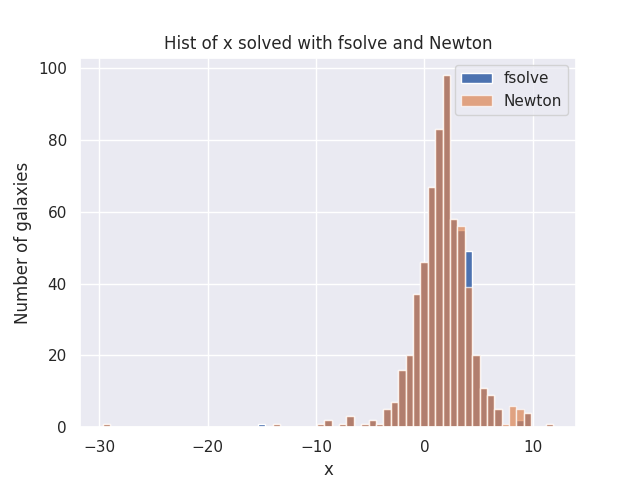
\includegraphics[width=.9\linewidth]{figure/x-hist.png}
\end{center}


\begin{verbatim}
<QTable length=607>
name  dtype     class       mean    std     min      max   n_bad
---- ------- ------------ ------- ------- -------- ------- -----
 x_f float64 MaskedColumn 1.56101 2.88426 -29.6974 11.9164     0
 x_n float64       Column 1.66518 2.91771 -29.6974 11.9164     1
None
\end{verbatim}



\begin{center}
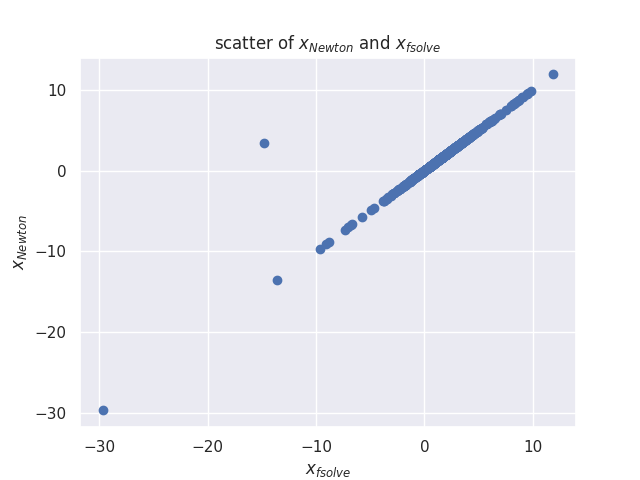
\includegraphics[width=.9\linewidth]{figure/x-scatter.png}
\end{center}


Since they are both pretty much the same, we can assume that the more compact is better, ie fsolve.

\subsubsection{Hist of A}
\label{sec:orgb536f22}

\begin{center}
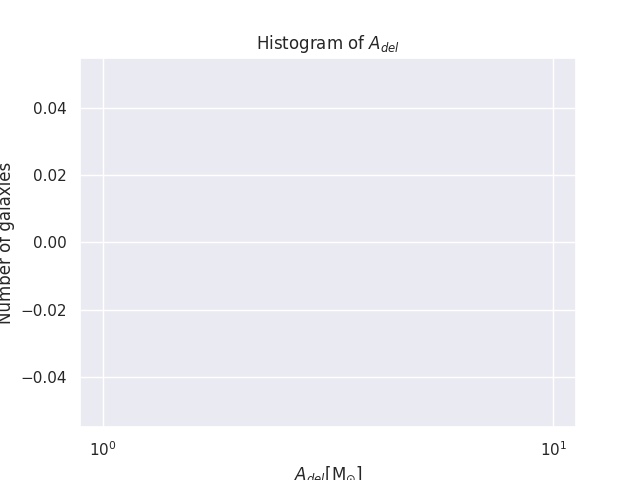
\includegraphics[width=.9\linewidth]{figure/A-hist.png}
\end{center}


\subsection{Calculating the t\textsubscript{sf} and \(\tau\) of the galaxies}
\label{sec:org06b21d0}

\begin{verbatim}
/home/dp/.local/lib/python3.10/site-packages/astropy/units/quantity.py:671: RuntimeWarning: overflow encountered in divide
name = tau
dtype = float64
unit = Gyr
class = Quantity
mean = 6.30189 Gyr
std = 77.365 Gyr
min = -1036.91 Gyr
max = 988.964 Gyr
n_bad = 0
length = 607
None
\end{verbatim}

\begin{verbatim}
<QTable length=607>
name  dtype    unit   class   n_bad
---- ------- ------- -------- -----
 A_n float64 solMass Quantity     1
 x_n float64           Column     1
None
\end{verbatim}



\url{None}

\subsubsection{{\bfseries\sffamily IDEA} Check to see if the almost inf points make any sense}
\label{sec:orgbb07f9e}

\subsection{{\bfseries\sffamily TODO} The gas depletion timescale \(\tau\)\textsubscript{g}}
\label{sec:orgae7d362}
What is the gas depletion timescale?



\subsection{{\bfseries\sffamily TODO} The theoretical SFR vs the observed}
\label{sec:org0f23e0c}


\section{{\bfseries\sffamily PROJ} The relations of the Masses}
\label{sec:org39c52db}
Since the aim of the paper is to find the SFR lets first understand and calculate the masses of the galaxies and see if we can find any relation with the SFR.

Pairplot with StellarMass, MHI, SFR\textsubscript{0} and av\textsubscript{SFR}, M26



\section{{\bfseries\sffamily TODO} The relations of the Data}
\label{sec:org0f3fcd7}

\subsection{{\bfseries\sffamily TODO} Luminosity and Masses}
\label{sec:org752f14a}

\subsection{{\bfseries\sffamily TODO} Variations in Star Formation Rates across the different masses}
\label{sec:org862160e}


\section{{\bfseries\sffamily TODO} Filling the Catalogue}
\label{sec:orgd74b51d}
\end{document}
